\begin{frame}[t]{V-JEPA: predicting representations instead of pixels}
  \begin{itemize}\itemsep0.26em
    \item[\textcolor{red}{$\blacktriangleright$}] \textbf{JEPA} = \emph{Joint Embedding Predictive Architecture}. Mask part of a video in space and time, then predict the \textbf{representation} of the masked region from the visible context.
    \item[\textcolor{red}{$\blacktriangleright$}] The loss lives in representation space, so there is no decoder and no pixel reconstruction. V-JEPA is trained \textbf{solely} on feature prediction: no pretrained image encoder, no text, no negative pairs, no reconstruction term.
    \item[\textcolor{red}{$\blacktriangleright$}] \textbf{Why bother:} pixels contain detail that is genuinely unpredictable (exact texture, noise). A reconstruction loss spends capacity on it; a representation-space loss can ignore it.
    \item[\textcolor{red}{$\blacktriangleright$}] Trained on 2M public videos, largest model ViT-H/16. Frozen-backbone evaluation: 81.9\% Kinetics-400, 72.2\% Something-Something-v2, 77.9\% ImageNet-1K.
    \item[\textcolor{red}{$\blacktriangleright$}] \textbf{The catch:} nothing here is action-conditioned, so V-JEPA predicts \emph{what comes next}, not \emph{what happens if I act}. That is what V-JEPA\,2 adds.
  \end{itemize}
  {\scriptsize Bardes et al., \href{https://arxiv.org/abs/2404.08471}{arXiv:2404.08471}.}
\end{frame}

\begin{frame}[t]{V-JEPA: video {JEPA}}
  \centering
  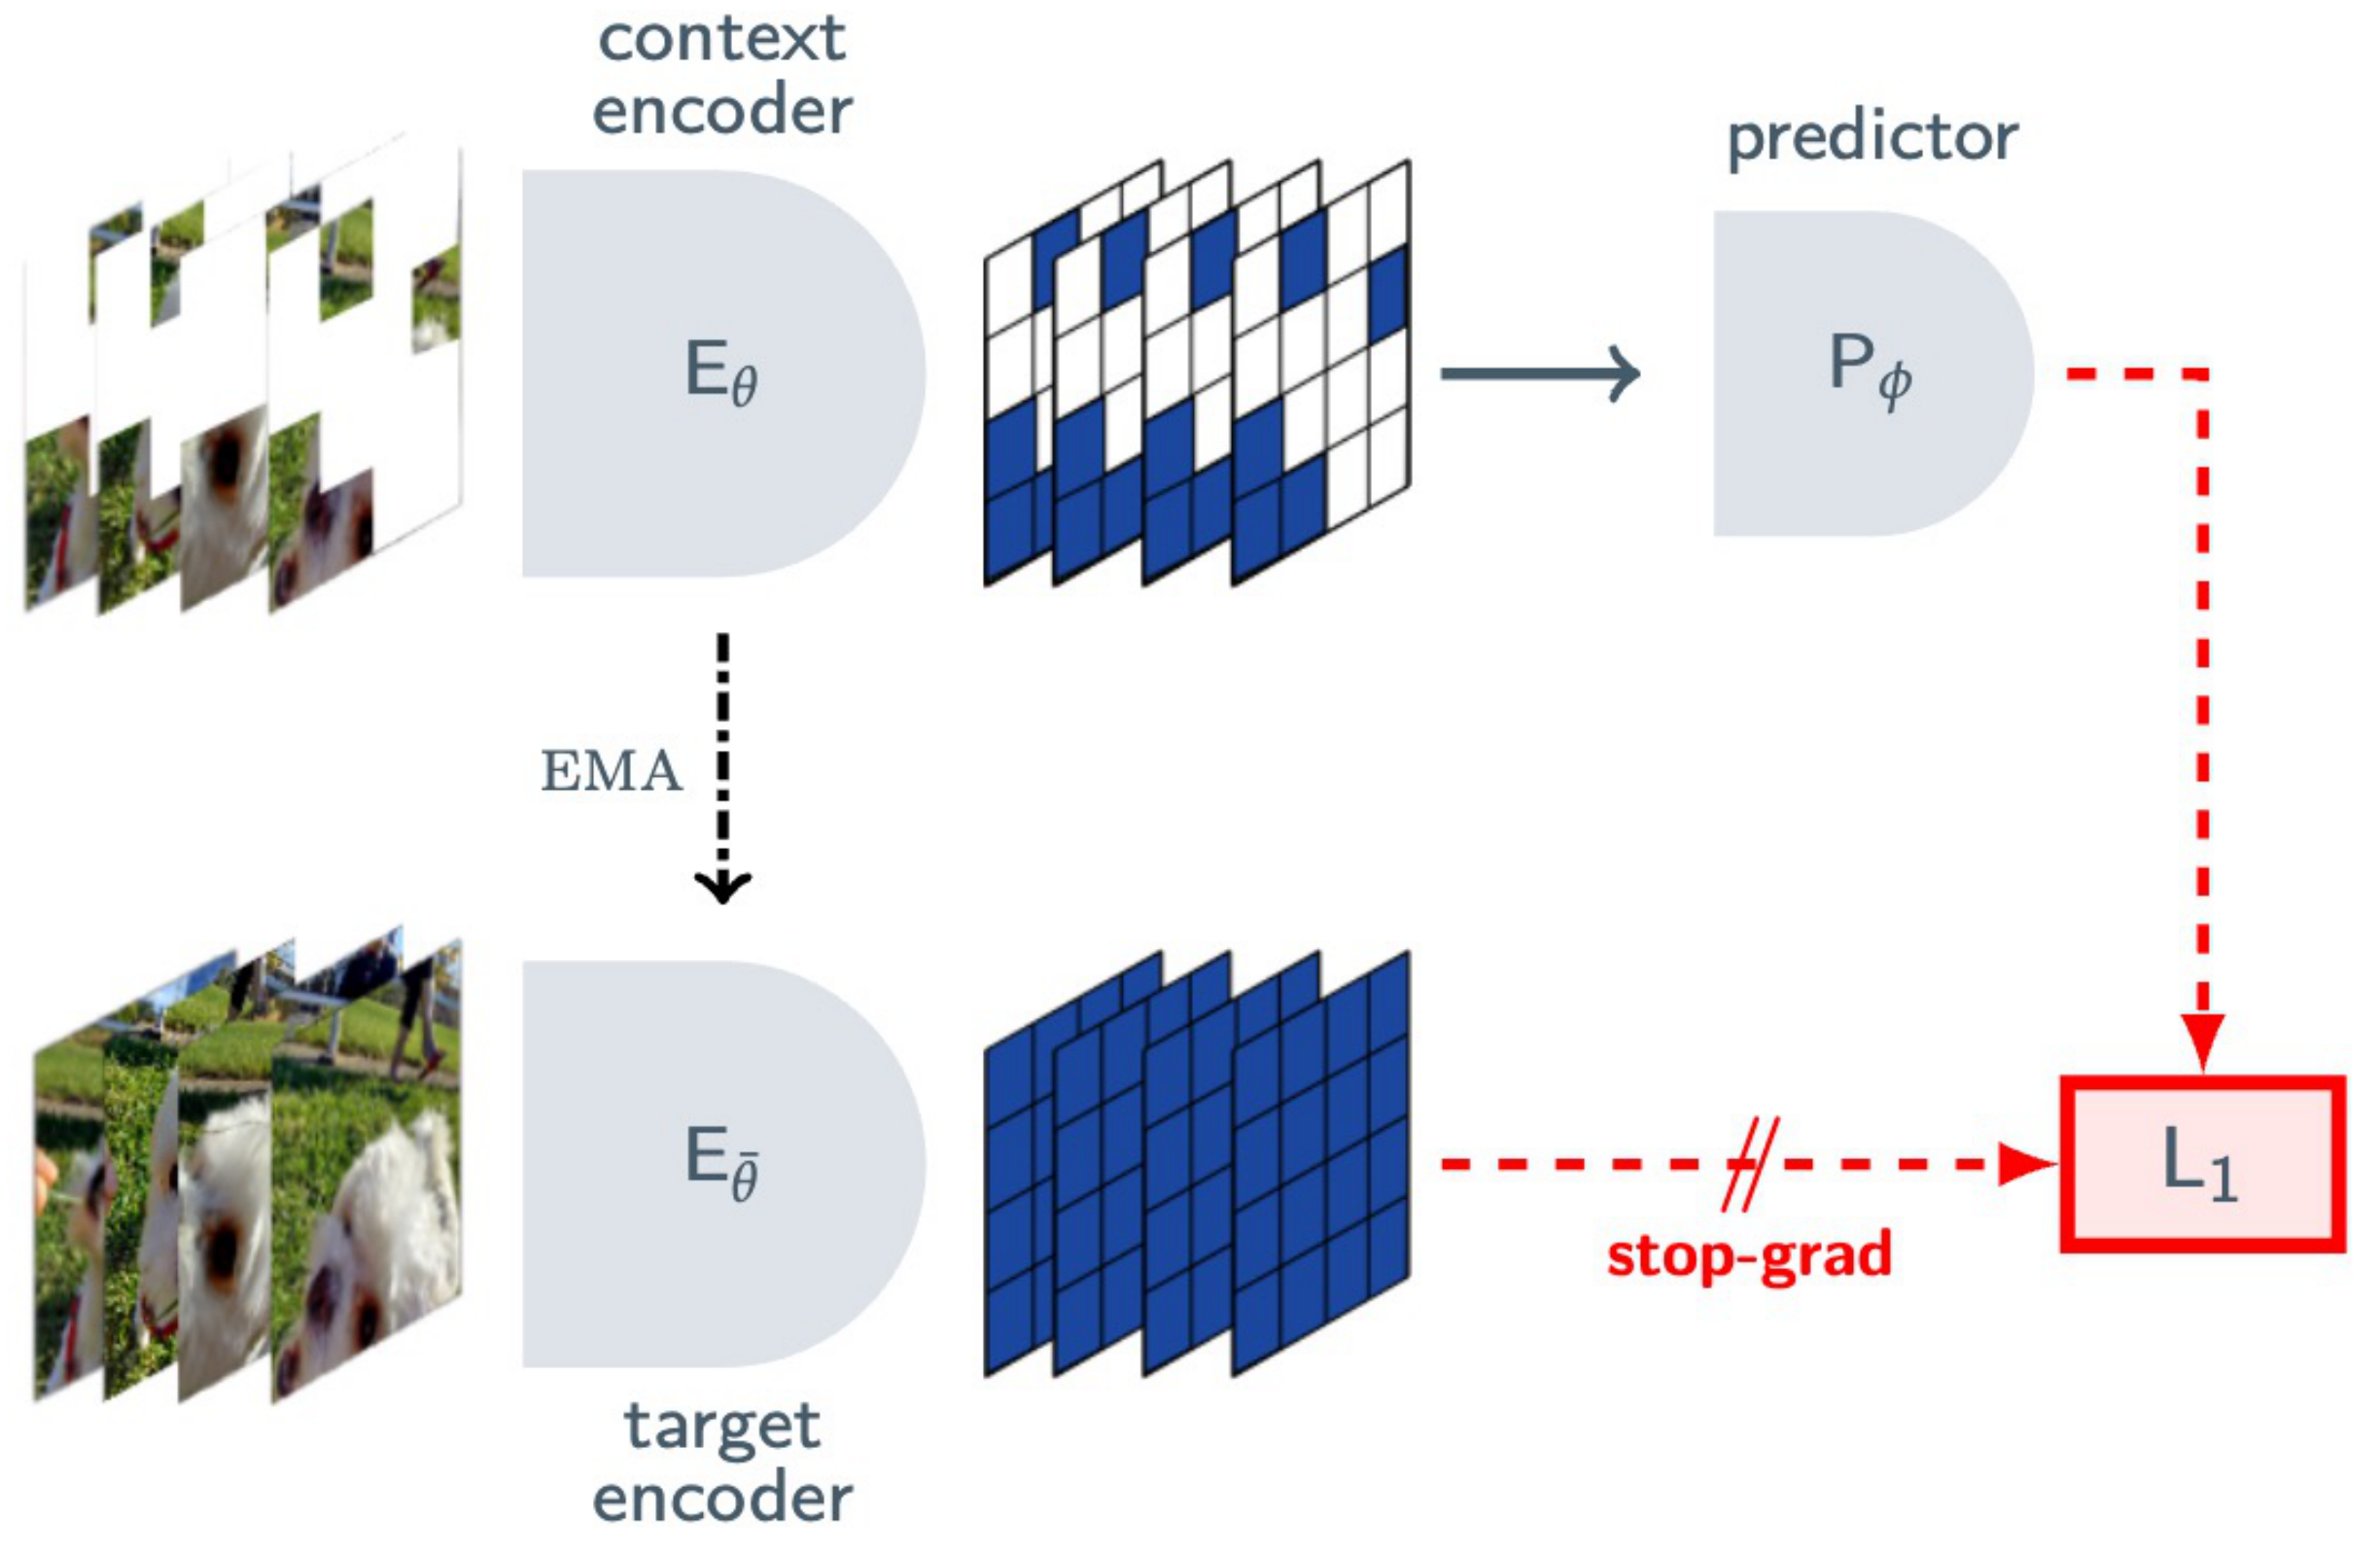
\includegraphics[width=\linewidth,height=0.82\textheight,keepaspectratio]{images/world-models/jepa_cs25_sl07_vjepa_bardes_2024.png}\\[0.08em]
  {\scriptsize Bardes et al., \href{https://arxiv.org/abs/2404.08471}{arXiv:2404.08471}. Image credit: \href{https://drive.google.com/file/d/1bF5Yfzf-FG5iNIAgsXn2DwVD3l3ymvZW/view}{CS25}.}
\end{frame}

\begin{frame}[t]{V-JEPA\,2: from prediction to planning}
  \begin{itemize}\itemsep0.3em
    \item[\textcolor{red}{$\blacktriangleright$}] \textbf{V-JEPA\,2-AC} is the action-conditioned variant: the predictor is additionally given the action, so it models the consequence of acting rather than just the continuation of a clip.
    \item[\textcolor{red}{$\blacktriangleright$}] It is post-trained on under \textbf{62 hours} of unlabelled robot video from the Droid dataset, which is small next to the 2M-video pretraining corpus.
    \item[\textcolor{red}{$\blacktriangleright$}] Given an image of the goal, the model is used for \textbf{planning}: search over candidate actions, roll them forward in latent space, and pick the one whose predicted representation lands nearest the goal.
    \item[\textcolor{red}{$\blacktriangleright$}] Deployed \textbf{zero-shot} on Franka arms for reaching, grasping and pick-and-place in environments not seen during training, with no task-specific reward or demonstration.
    \item[\textcolor{red}{$\blacktriangleright$}] This is the payoff of the latent route: planning needs a state you can compare against a goal, and it never needed the pixels.
  \end{itemize}
  \vspace{0.2em}
  {\scriptsize Assran et al., \emph{V-JEPA 2: Self-Supervised Video Models Enable Understanding, Prediction and Planning};
  \href{https://arxiv.org/abs/2506.09985}{arXiv:2506.09985}.}
\end{frame}

\begin{frame}[t]{V-JEPA\,2: action-conditioned latent prediction}
  \centering
  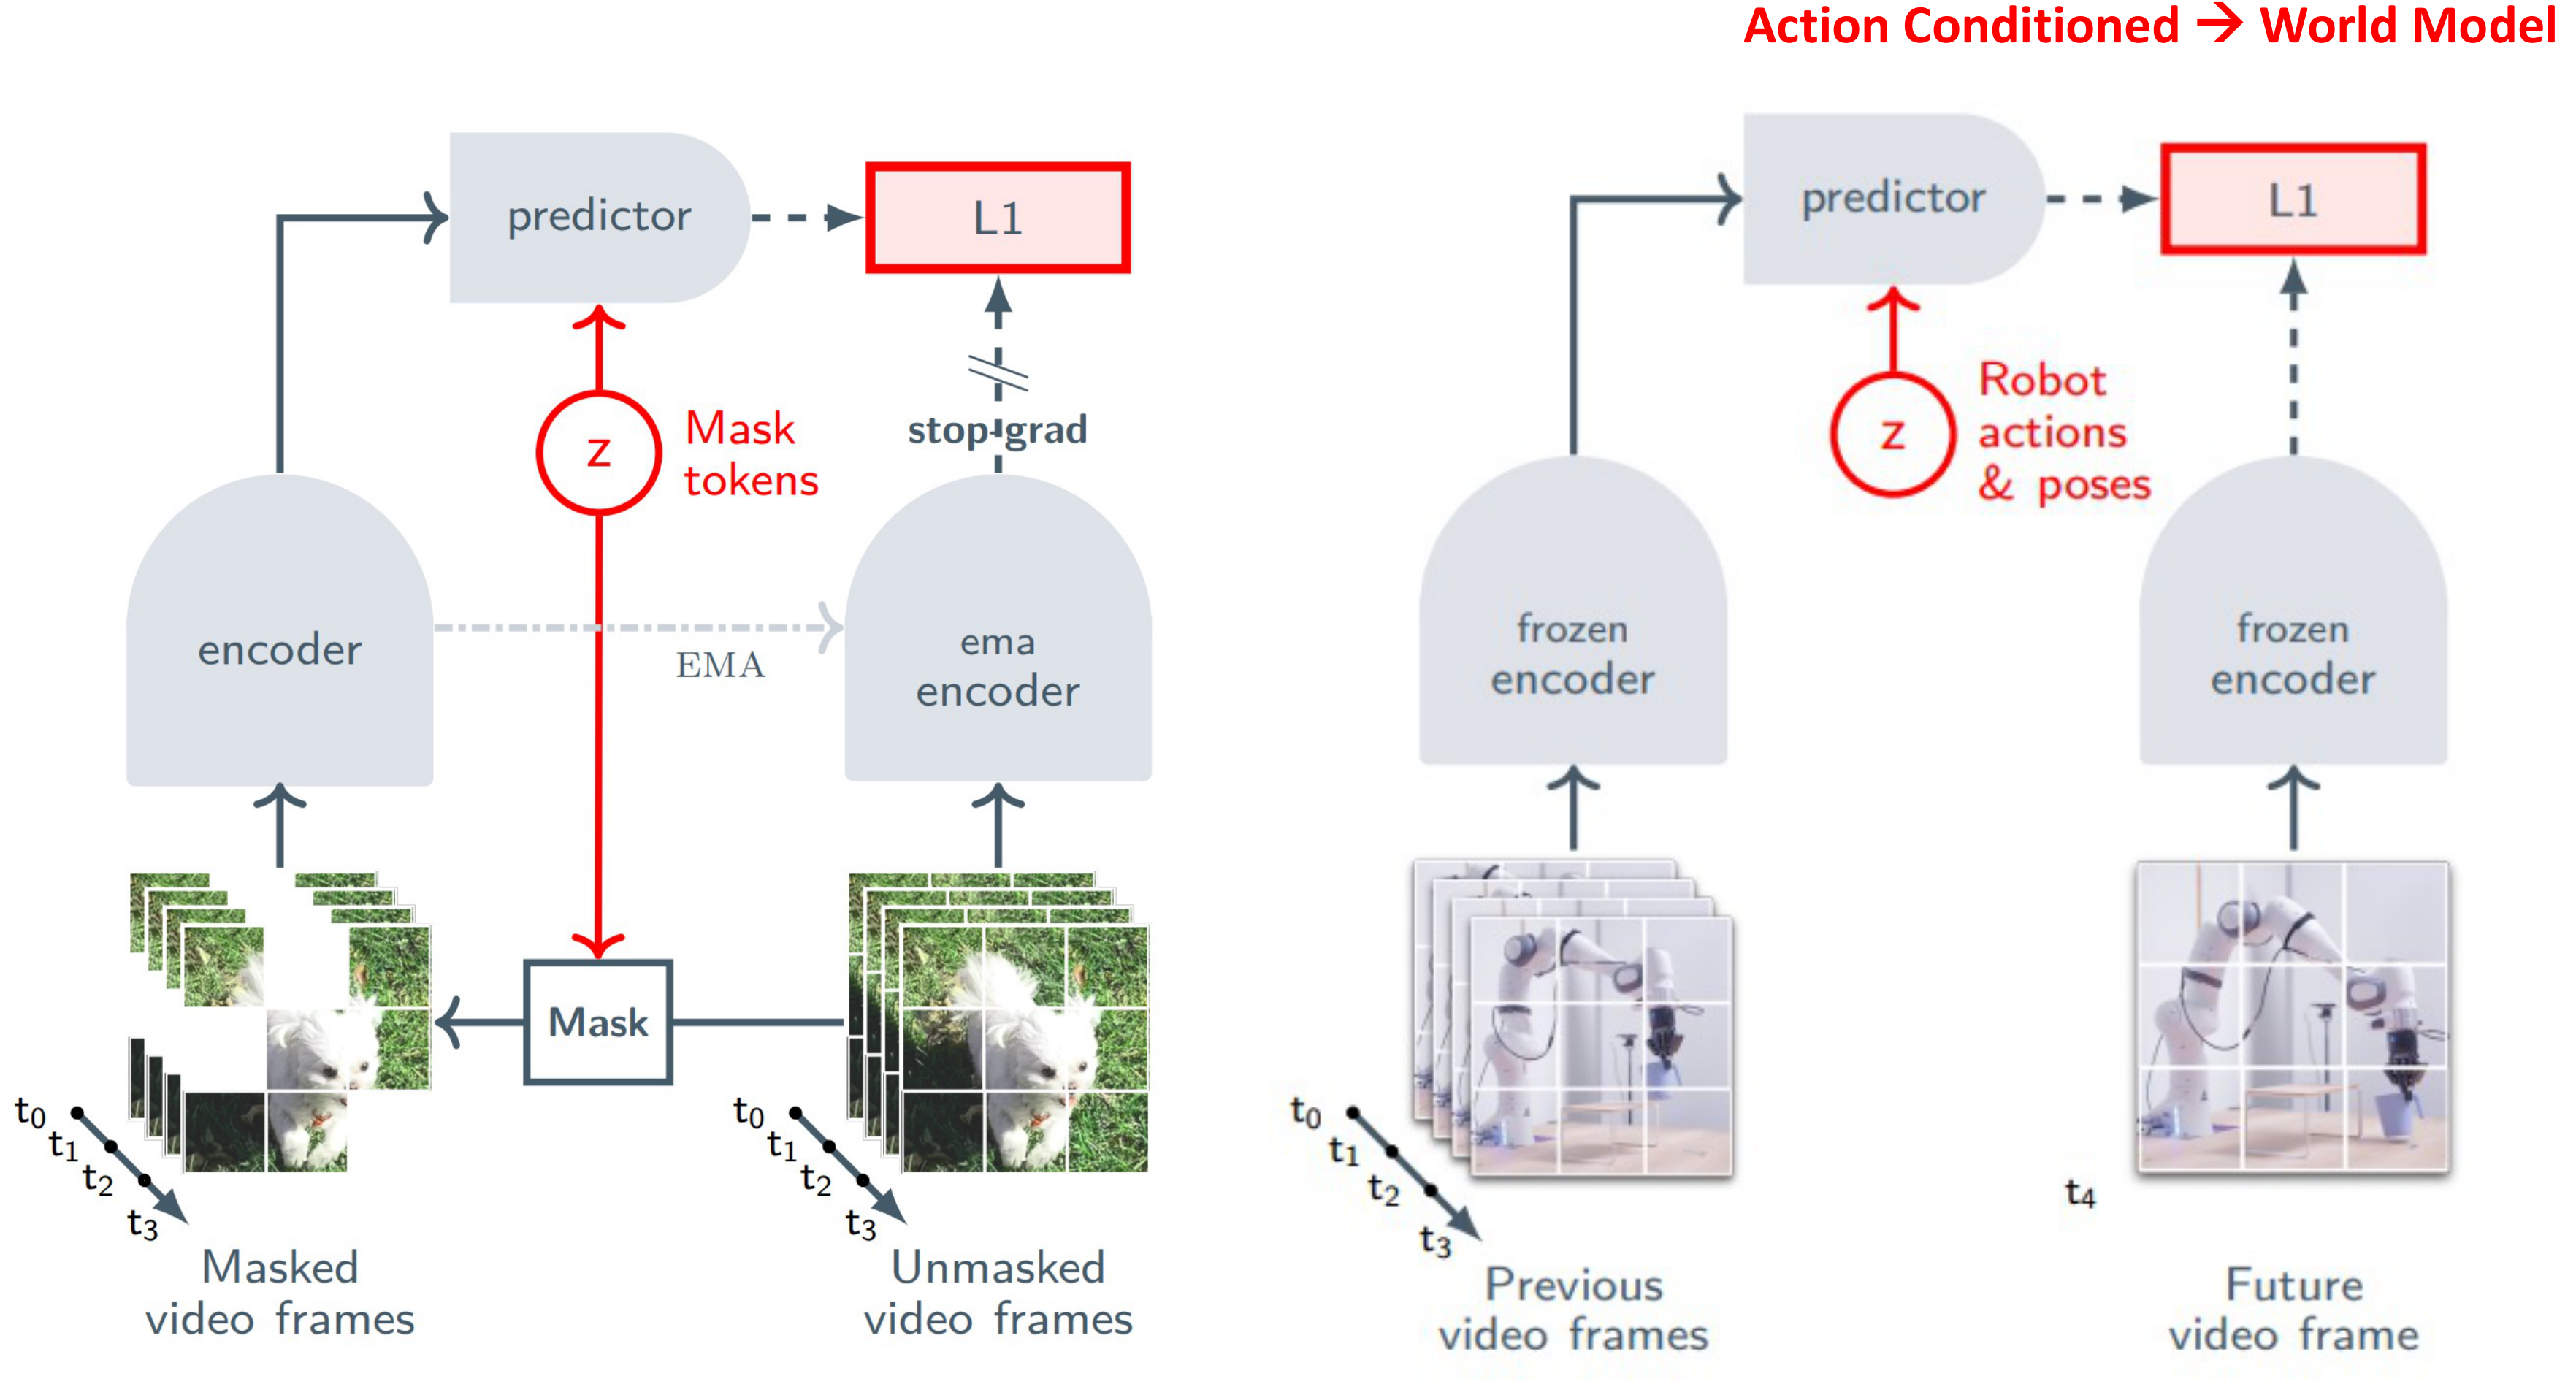
\includegraphics[width=\linewidth,height=0.74\textheight,keepaspectratio]{images/world-models/jepa_cs25_sl08_vjepa2_action_world_model.png}\\[0.04em]
  {\scriptsize Assran et al., \href{https://arxiv.org/abs/2506.09985}{arXiv:2506.09985}. Image credit: \href{https://drive.google.com/file/d/1bF5Yfzf-FG5iNIAgsXn2DwVD3l3ymvZW/view}{CS25}.}
\end{frame}
